
%% bare_conf.tex
%% V1.4
%% 2012/12/27
%% by Michael Shell
%% See:
%% http://www.michaelshell.org/
%% for current contact information.
%%
%% This is a skeleton file demonstrating the use of IEEEtran.cls
%% (requires IEEEtran.cls version 1.8 or later) with an IEEE conference paper.
%%
%% Support sites:
%% http://www.michaelshell.org/tex/ieeetran/
%% http://www.ctan.org/tex-archive/macros/latex/contrib/IEEEtran/
%% and
%% http://www.ieee.org/

%%*************************************************************************
%% Legal Notice:
%% This code is offered as-is without any warranty either expressed or
%% implied; without even the implied warranty of MERCHANTABILITY or
%% FITNESS FOR A PARTICULAR PURPOSE! 
%% User assumes all risk.
%% In no event shall IEEE or any contributor to this code be liable for
%% any damages or losses, including, but not limited to, incidental,
%% consequential, or any other damages, resulting from the use or misuse
%% of any information contained here.
%%
%% All comments are the opinions of their respective authors and are not
%% necessarily endorsed by the IEEE.
%%
%% This work is distributed under the LaTeX Project Public License (LPPL)
%% ( http://www.latex-project.org/ ) version 1.3, and may be freely used,
%% distributed and modified. A copy of the LPPL, version 1.3, is included
%% in the base LaTeX documentation of all distributions of LaTeX released
%% 2003/12/01 or later.
%% Retain all contribution notices and credits.
%% ** Modified files should be clearly indicated as such, including  **
%% ** renaming them and changing author support contact information. **
%%
%% File list of work: IEEEtran.cls, IEEEtran_HOWTO.pdf, bare_adv.tex,
%%                    bare_conf.tex, bare_jrnl.tex, bare_jrnl_compsoc.tex,
%%                    bare_jrnl_transmag.tex
%%*************************************************************************
\documentclass[conference]{IEEEtran}
% Add the compsoc option for Computer Society conferences.

\ifCLASSINFOpdf
  \usepackage[pdftex]{graphicx}
  \graphicspath{{img/}}
  \DeclareGraphicsExtensions{.pdf,.jpeg,.png}
\else
  \usepackage[dvips]{graphicx}
  \graphicspath{{../img/}}
  \DeclareGraphicsExtensions{.eps}
\fi

\usepackage[cmex10]{amsmath}

% *** ALIGNMENT PACKAGES ***
%
%\usepackage{array}
% Frank Mittelbach's and David Carlisle's array.sty patches and improves
% the standard LaTeX2e array and tabular environments to provide better
% appearance and additional user controls. As the default LaTeX2e table
% generation code is lacking to the point of almost being broken with
% respect to the quality of the end results, all users are strongly
% advised to use an enhanced (at the very least that provided by array.sty)
% set of table tools. array.sty is already installed on most systems. The
% latest version and documentation can be obtained at:
% http://www.ctan.org/tex-archive/macros/latex/required/tools/


% IEEEtran contains the IEEEeqnarray family of commands that can be used to
% generate multiline equations as well as matrices, tables, etc., of high
% quality.




% *** SUBFIGURE PACKAGES ***
\ifCLASSOPTIONcompsoc
  \usepackage[caption=false,font=normalsize,labelfont=sf,textfont=sf]{subfig}
\else
  \usepackage[caption=false,font=footnotesize]{subfig}
\fi
% subfig.sty, written by Steven Douglas Cochran, is the modern replacement
% for subfigure.sty, the latter of which is no longer maintained and is
% incompatible with some LaTeX packages including fixltx2e. However,
% subfig.sty requires and automatically loads Axel Sommerfeldt's caption.sty
% which will override IEEEtran.cls' handling of captions and this will result
% in non-IEEE style figure/table captions. To prevent this problem, be sure
% and invoke subfig.sty's "caption=false" package option (available since
% subfig.sty version 1.3, 2005/06/28) as this is will preserve IEEEtran.cls
% handling of captions.
% Note that the Computer Society format requires a larger sans serif font
% than the serif footnote size font used in traditional IEEE formatting
% and thus the need to invoke different subfig.sty package options depending
% on whether compsoc mode has been enabled.
%
% The latest version and documentation of subfig.sty can be obtained at:
% http://www.ctan.org/tex-archive/macros/latex/contrib/subfig/




% *** FLOAT PACKAGES ***
%
%\usepackage{fixltx2e}
% fixltx2e, the successor to the earlier fix2col.sty, was written by
% Frank Mittelbach and David Carlisle. This package corrects a few problems
% in the LaTeX2e kernel, the most notable of which is that in current
% LaTeX2e releases, the ordering of single and double column floats is not
% guaranteed to be preserved. Thus, an unpatched LaTeX2e can allow a
% single column figure to be placed prior to an earlier double column
% figure. The latest version and documentation can be found at:
% http://www.ctan.org/tex-archive/macros/latex/base/


%\usepackage{stfloats}
% stfloats.sty was written by Sigitas Tolusis. This package gives LaTeX2e
% the ability to do double column floats at the bottom of the page as well
% as the top. (e.g., "\begin{figure*}[!b]" is not normally possible in
% LaTeX2e). It also provides a command:
%\fnbelowfloat
% to enable the placement of footnotes below bottom floats (the standard
% LaTeX2e kernel puts them above bottom floats). This is an invasive package
% which rewrites many portions of the LaTeX2e float routines. It may not work
% with other packages that modify the LaTeX2e float routines. The latest
% version and documentation can be obtained at:
% http://www.ctan.org/tex-archive/macros/latex/contrib/sttools/
% Do not use the stfloats baselinefloat ability as IEEE does not allow
% \baselineskip to stretch. Authors submitting work to the IEEE should note
% that IEEE rarely uses double column equations and that authors should try
% to avoid such use. Do not be tempted to use the cuted.sty or midfloat.sty
% packages (also by Sigitas Tolusis) as IEEE does not format its papers in
% such ways.
% Do not attempt to use stfloats with fixltx2e as they are incompatible.
% Instead, use Morten Hogholm'a dblfloatfix which combines the features
% of both fixltx2e and stfloats:
%
% \usepackage{dblfloatfix}
% The latest version can be found at:
% http://www.ctan.org/tex-archive/macros/latex/contrib/dblfloatfix/




\usepackage{url}
\usepackage{glossaries}

\newacronym{APICSS}{APICSS}{Art Painting Image Color Semantics}
\newacronym{RGB}{RGB}{Red, Green, Blue}
\newacronym{HSL}{HSL}{Hue, Saturation, Luminance}
\newacronym{HSV}{HSV}{Hue, Saturation, Value}
\newacronym{PCA}{PCA}{Principal Component Analysis}
\newacronym{t-SNE}{t-SNE}{t-Distributed Stochastic Neighbor Embedding}

% correct bad hyphenation here

\begin{document}

\title{Digital Analysis of Paintings}

\author{\IEEEauthorblockN{Alexander David Brown}
\IEEEauthorblockA{Computer Science,\\
Aberystwyth University,\\
Penglais,
Aberystwyth,\\
Ceredigion,\\
Wales SY23 3DB\\
Email: adb9@aber.ac.uk}
}

\maketitle

\begin{abstract}
%TODO Write this once the paper is complete
\end{abstract}

% no keywords

\IEEEpeerreviewmaketitle

\section{Introduction}
Digital image processing is a field which encourages the crossover of different
scientific disciplines, often biological research and computer vision align to
automate the collection and analysis of plant growth. However, art and
computing are fields which, at first glance, have very little in common.

But a deeper look unveils a plethora of different avenues from detecting
forgeries to being able to date an artists work within a catalogue of their
known pieces.

This survey paper will unearth some techniques which can be applied to the
digital analysis of paintings, as well as existing research which has already
applied computer vision to the field of art.

\section{Colour Analysis}
Digital images are typically considered to be a matrix of pixels, where each
pixel contains information about the colour of that place in the image. 

Colours can be represented in numerous different ways, but are typically three
to four bytes; for example the \gls{RGB} colour space uses one byte for the
levels of red, one for green and one for blue. The fourth byte is unlikely to
be considered in artwork as it usually represents the transparency, known as
the alpha channel, of the pixel.

A single byte colour space purely focuses on the intensity of a pixel, in
actuality this represents a grayscale image.

Analysing colour is the base of all analysis techniques in image processing,
the value(s) of a pixel with regards to its location and neighbours can be used
to build up some very complex knowledge about the image. This section will deal
specifically with the colours which an artist uses within their work, such as
looking at the distribution of colours across a work, rather than using colour
information to determine textures.

\subsection{Colour Distribution}
% Paper 7

The distribution of colour across an image can give a surprising amount of
information about that image, especially given that colour is very subjective
to an individual.

Ivonna, Stanchev and Dimitrov investigated the colour
distribution within the works of over 100 artists for several different
countries and periods, using a system named \gls{APICSS}\cite{ivanova2008analysis}.

Existing systems already statistically analysed colours within an image and
some even used classifiers, typically a naive Bayesian classifier as it fits
well with statical methods, to perform extra analysis.

Unlike these existing system, \gls{APICSS} focused primarily on the \gls{HSL}
colour space as it is the closest representation to an artist's colour wheel.
\gls{HSV} was also considered, but because the lightness is not symmetrical
within the \gls{HSV} colour space, it is less useful for direct comparison.

As with any system involving classification, a feature space is needed to
represent an item within the data set. In the case of \gls{APICSS} the feature
space is three dimensional, one for each of the values in the colour space.

From this, a distance measure (in this case Euclidean distance) can be used to
compare different items.

\gls{APICSS} also take into account some of the metadata attached to each
painting, such as the movement and sub-movement during which the painting was
created. This allows for more statistical analyses to be performed on sub-sets
of the data set.

\gls{APICSS} appears to be a good system, which considers both metadata and
analysis gained from the digitisation of artwork. The paper considers a wide
range of artists and periods.

However, the use of a lossy image format (JPEG) could potentially skew the
results. The system itself is very basic, especially if it only considers
\gls{HSL} and metadata. This is further compounded by only considering thirteen
colours within the Hue (twelve separate colours and one achromatic).

Despite having a decent sized data set overall, some of the categories have
relatively small items within them.

Overall \gls{APICSS} is a good application of existing research, but uses very
basic analysis techniques on the images themselves.


\subsection{Pigment Mapping}
% Paper 3
Colour analysis can also give a glimpse into the colour pigments the artist
used to create the work. Using a database of known oil pigments and
\textit{a priori} knowledge, it is possible to work out which pigments are used
in a painting, and also to be able to show which parts of the painting are made
up from which pigment\cite{zhao2008investigation}.

This is done through a process known a multispectral imaging, the process of
capturing a different frequencies to provide a different spectrum of light and
enable more analysis.

This technique is especially powerful for segmenting different pigments in an
image as each pigment is made up of a different substance.

Because this process requires both hardware and software it make a large
different whether the materials a work is made up of are known. When known it
can be possible to find the combinations of these materials at a given point
and their concentrations.

When the materials are unknown, extra processing is required to decide which
materials the painting comprises of. This process uses spectral processing but
also requires prior knowledge of the artist and art tools.

In the experimental results this paper provides, the latter is achieved by a
study of another of Van Gogh's works from the same time.

Pigment mapping across every pixel is a costly operation in terms of memory and
CPU time. This research makes a reasonable assumption that a similar colour
will have been painted using similar pigments to reduce the amount of pigment
mapping which occurs. This does lead to unwanted side-effects, but the only way
to combat these is to increase the number of pixels which pixel-mapping.

To reduce the number of pixels considered for pigment mapping the image is
first partitioned into a number of smaller images to reduce processing time on
the next steps

Each of these partitioned regions is then split into a number of clusters based
on the colours of the pixels. This was done using supervised and unsupervised
algorithms. The unsupervised algorithm was very sensitive and had long running
times whilst the supervised algorithm requires a human observer.

Finally pixels within these clusters were then selected based on the similarity
of pixels within the cluster, the clusters and partitioned images can then be
stitched back together and rendered based on the pigment maps.

This research could be incredibly useful if it could be applied to the analysis
of artwork and the field of multispectral analysis has already had a lot of
success in other fields.

However, because this is both a hardware- and software-based system, it may not
be something which can be used with regularity as it requires the physical
presence of the paintings, which not all artwork analysis researchers have
access to.

It also requires a lot of a priori knowledge of the artist and calculating the
materials a painting consists of may be a difficult, if not impossible task,
depending on the artist.

In conclusion, this technique can provide a very powerful analysis of a
painting, but at the cost of requiring specialised hardware, the physical
painting and expert knowledge about the artist, so is a very manual process.

This technique could be improved by using a less naive clustering unsupervised
algorithm to remove some of the need for human intervention, but the need for
the physical painting will always be a limiting factor of this work.

\subsection{Difference Visualisation}
% Paper 6
Another approach to colour is to visualise the difference between two or more
different images, this is particularly of use for comparing different versions
of the same image - the original to a famous forgery, for example.

Image fusion is the process of combining two different images and has recently
been applied to artwork\cite{blazek13image}. In this research, a technique for
showing the differences between two or more images which can show positive,
negative and zero difference between the images, whilst maintaining regions of
interest between the two images. 

The method for doing this uses the CIELAB colour space, which maps more
faithfully to human vision than other colour spaces. However, because of the
limitations displaying the images, they are converted to \gls{HSV} before they
are displayed.

A hue for both the positive and negative difference values is selected by the
user as a vector, then the difference in the \gls{HSV} saturation of the two
images is then computed into CIELAB, where it is an angle between the
aforementioned colour vector.

Finally this is converted into \gls{HSV}, where the Hue represents the sign of
the computed image, the saturation the absolute distance and the value the
average value of intensities of the compared image at that pixel.

The authors claim this fusion improves the comprehension of the difference
visualisation of images and that it makes identifying regions of interest
faster and more precise, but provide no experimental results to prove this
other than the fused image result of four different copies of the same artwork.

This does keep the original image intact (albeit in grayscale with differences
highlighted).

This does only provide visualisation rather than analysis, but could potential
be used as part of a larger system to build more complex analysis techniques.
This might be especially useful to pick up difference between an original and a
derivative work or forgery.

At current, the images must be aligned and scaled manually, but this process
could be automated trivially.

This research appears to be of very limited use, but when used within as a part
of a larger system could provide some very interesting analysis which could be
used to train classifiers to detect forgeries, etc. but this still has limited
scope.

\section{Texture Analysis}
Paintings are somewhat unlike the normal subject for image processing, whilst
most images are either simple two dimensional images, or two dimensional slices
of a three dimensional object. Paintings often thought of as two dimensional,
but with many paint types these paintings become three dimensional.

This aspect is lost in the digitisation of the painting; but there are still
ways of analysing the texture of the image by analysing the colour of the
image. Quite often, this is as effective on a one dimensional colour space as
it is on a three dimensional one.

Filters can be passed over an image to gather basic information such as
direction of lines within the paintings. More complex techniques for analysing
texture involve using wavelets and considering nearby pixels.

\subsection{Steerable Filters}
% Paper 12

For techniques which involve applying a filter to decide the direction of a
line within a picture, one often needs to be able to change or rotate the
filter by varying amounts of degrees. This principal is often described as
steering a filter and an efficient technique for doing so is described in 
\cite{freeman91design} in both two and three dimensional space.

This technique involves finding a function of $x$ and $y$ which steers a filter

% TODO I'm struggling to understand this one...

\subsection{Gabor Filters}
% Paper 13

% TODO Again, another complex one :-(

\subsection{Histograms of Edge Orientated Gradients}
% Paper 8

A method for analysing the texture over an image to to create a histogram which
contains the orientation of all the gradients over an image. This technique has
been applied to the field of human detection\cite{dalal05histograms}, but is
also useful when applied to the realm of digital analysis of artwork as well.

A lot of the methodology for human detection involves the normalisation and
classification, but does include some useful information about the practises of
generating histograms of edge-orientated gradients. The gradients are computed
using a variety of discrete derivative masks combined with degrees of Gaussian
smoothing, although the results show that Gaussian smoothing and larger masks
damage the performance.

Each pixel is then binned according to a weighted vote from the mask, then each
vote is accumulated into orientation bins in local regions, which could be
rectangular or radial.

These orientation bins were evenly spaced across $0-\pi$ unsigned bins or
$i-2\pi$ signed bins. This is significant to note an orientation $\theta$ below
$\pi$ is often thought of as equivalent to $\theta + \pi$ in image processing.

Normalisation is then applied to reduce the effects of local contrast and is
good for performance in the field of human detection. For artwork this may be
less useful as these features are of importance.

This research shows very good experimental results of large, popular data sets
and beats all of the existing techniques on false positives (although no data
for false negatives is shown).

Although this research does not directly relate to the field of digital
analysis of artwork, it has been used to generate some interesting
analysis\cite{brown13can} although not all of the technique was applied in that
research.

The use of this research is the ability to store orientation data in
histograms, which are very easy to process digitally.

In conclusion, this technique provides a powerful analysis technique and the
experimental results on several decent sized data sets to prove this. Although
not all of the technique is useful or applicable to the digital analysis of
paintings, the parts which are have been successfully used in research into
artwork.

\subsection{Multifractal Classification}
% Paper 5

Another analysis paradigm is fractal geometry which is based on the idea that
all analysis performed on an image at difference scales are equally important
and that the richest information can be found in the mechanisms which relate
them to one another.

Because of this, fractal tools can be used to analyse contours and textures of
images.

Multifractal analysis concentrates on the use of processing tools which
describe the fluctuations within regular regions of an object which at
different scales.

Until recently multifractal analysis was rarely applied to image processing
problems, but with the breakthrough in an efficient formulation of
multifractal analysis obtained through wavelet leaders.

The use of wavelet leader multifractal analysis has been used to explore
painting texture classification\cite{abry2013van}.

Image processing is a field which has grown out of signal processing; an image
can actually be thought of as a two-dimensional signal, which allows existing
signal processing techniques to be applied to them. In early days of image
processing the Fourier transform was often used to decompose images into
signals. In more recent years wavelets and transforms using wavelets have
become more popular, as they can provide all the features of a Fourier
transform, but also provide localised time information, as well as localised
frequency information.

In the case of images, localised time information maps to the location within
an image.

In this research, a 2D discrete wavelet transform is applied to the image to
gather the wavelets coefficients, normalising the image to the correct form
needed for the definition of wavelet leaders.

These coefficients enable a definition of the global regularity of the image.

To allow image classification across different scales, one needs a dyadic
space; a space in which there are a collection of regions of different scales,
where a region at one scale can also be viewed as the union of regions in a
smaller scale. Figure~\ref{fig:dyadic-image}\footnote{The photograph is
property of the U.S. Federal Government, and is therefore in the public
domain} shows an example of this where the large regions show only a pixalated
view of the image and the smallest the individual pixels of the image.

\begin{figure}[ht]
\centering
\subfloat[$C=8$]{
\includegraphics[width=0.1\textwidth]{dyadic_2.png}}%
\hspace{.2in}%
\subfloat[$C=32$]{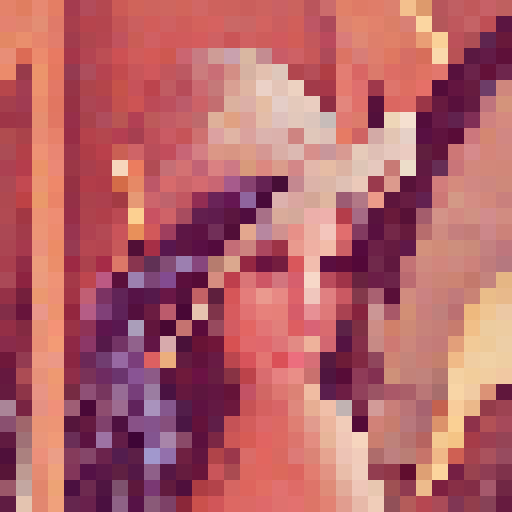
\includegraphics[width=0.1\textwidth]{dyadic_4.png}}%
\hspace{.2in}%
\subfloat[$C=128$]{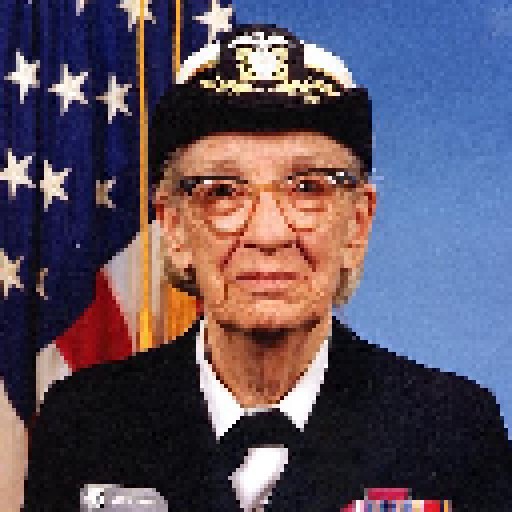
\includegraphics[width=0.1\textwidth]{dyadic_8.png}}%
\hspace{.2in}%
\subfloat[$C=512$ (Original Size)]{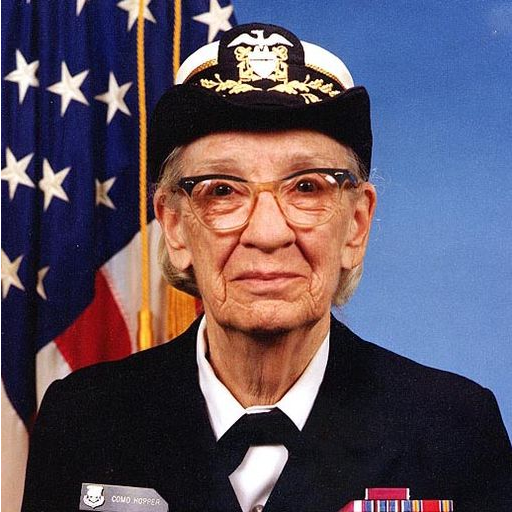
\includegraphics[width=0.1\textwidth]{dyadic_16.png}}%
\caption{Example of dyadic space using an image of Grace Hopper (512x512
pixels) at different dyadic scales ($C$), note how the picture becomes less
pixalated at higher scales}
\label{fig:dyadic-image}
\end{figure}

A natural interpretation of multifractal analysis needs to be based on wavelet
leaders, which allows an estimation of the multifractal spectrum of an image.
The wavelet coefficients at finer scales within a small neighbourhood are used
to renormalise the wavelet coefficients at a given scale.

This is all theoretically very sound, but in practise it cannot be used on
paintings without some modifications, mainly due to the fact that digital
objects do not have an infinite resolution. So the analysis is slightly
simplified to account for this to provide a fair estimation of the real
analysis.

This technique was applied to several different works, but the most interesting
of there was the Princeton experiment, where an artist produced seven distinct
small paintings using different materials. Two weeks later the artist was asked
to produce replicas as close to the original as possible.

Both the originals and replicas were scanned at a very high resolution to allow
this analysis to be as detailed as possible.

The results showed that, systematically, the textures of the replicas were
globally more regular and smoother than the originals. However, it should be
noted that getting these results required the expert selection of sections to
analyse and the a posteriori selection of the range of scales for wavelet
leaders. 

With promising results shown from this experimentation, attention was turned to
a norm for painting analysis: Van Gogh. Rather than consider the global state
of the canvas, each image was split into smaller sections for the analysis, as
paintings very rarely have the same texture globally.

This analysis was used to try and place paintings in a date region and detect
forgeries. The results shown for dating paintings into a period show some
promising results, where the majority of paintings were correctly clustered
into their correct periods. For detecting forgeries the results are promising,
but one forgery slips by when it was noticed by experts.

This technique is agnostic to the colour space and the authors do apply it to
several different colour spaces, including black-white intensity, \gls{RGB} and
\gls{HSL}. 

There is a lot of expert knowledge which cannot be automated or, where it can
be, is very arbitrary such as blindly selecting patches.

The results from the Princeton experiments are promising, but the results are
very sensitive to the material of the canvas as well as the tools used, whilst
this might be use for detecting forgeries, there might be situations where this
isn't desired.

The images the authors use are high resolution (800 DPI) and they note that a
lower resolution makes it difficult to decide on the range of scales which are
involved.

The data sets used are relatively small and, although they increase the
knowledge by taking multiple patches from the Van Gogh paintings, but for the
results they show only individual paintings are considered. One could easily
question the validity of their results based on this.

In conclusion this is a very complex but powerful technique which is actually
applying theoretical concepts to perform some interesting analysis and
classification. However, the sensitivity of the technique and with the need for
expert and a posteriori decisions do limit the real application of this
research.

\subsection{Texton-Based Analysis}
% Paper 11

Analysis of texture can also be performed with the help of a set of small
patches, or textons, relating to the texture of the image. An interesting
approach is to learn a variety of these textons from example images and then
look at a histogram of the frequencies of these textons on the images to
classify\cite{van2010texton}.

Segmentation of brushstrokes is, understandably, difficult - especially
digitally where the image is usually only two dimensional, but one can consider
the texture of the painting with more ease and can provide a good insight into
the artists style.

Filters are becoming less popular for painting analysis as the filter often
normalises the image to a certain extent in the process of analysis. Other
approaches like wavelets and pixel-based representations, such as texton
approaches, are becoming more popular to avoid this issue.

It should be noted that whilst textons are a building block of the text of an
image, they are not identical to brushstrokes.

To construct the codebook of textons, 5000 patches are selected in random
locations from each painting in the training set. These patches are then
clustered and the most exemplary patch (the central patch) is selected as the
most representative for that cluster.

From this codebook it is then possible to generate a histogram for any image
which estimates the distribution of these textons across the image. The
histogram is created by applying a sliding window across the painting and
selecting the nearest texton in euclidean space to the window. Finally the
histogram is normalised to sum up to 1.

The authors note that these histograms could be built up for different sizes of
textons to increase the feature space available for analysis, for their own
experiments they use six different scales of texton.

Because the aim of this research was to work closely with experts in the field,
the authors also came up with a method for visualising this information. For an
image processing system this may not be required, but could be used to extract
more useful information from the analysis.

Because of the high dimension space it is necessary to reduce the
dimensionality of the results to allow it to be human readable. Usually this
would be performed by \gls{PCA}, but the way in which the data is structured,
\gls{PCA} is too lossy for texton histograms; it has a linear nature whist the
texton histograms may be high-dimensionally non-linear and it focuses on
preserving the global structure rather than local structure of high-dimensional
points.

There are other techniques which might have been applied to solve these
problems, but the authors found some shortcomings with these techniques which
would have made real-life visualisation difficult.

To cope with this, a new method for dimensionality reduction was invented:
\gls{t-SNE}. This method hinges around keeping
the conditional probabilities between the high and low dimension spaces
similar.

Interestingly, in the experiments \gls{PCA} was first use to reduce the
dimensions down to 50, and then \gls{t-SNE} was
used to reduce down to two dimensions. Suggesting that, for very high dimensions,
\gls{t-SNE} is not very effective.

The results on 117 high-resolution grayscale Van Gogh paintings show that most
of the non-Van Gogh paintings appear on the peripheries of the visualised
two-dimensional graph, apart from two specific forgeries: the Wacker forgery
which had fooled experts for many years, but can successfully be found by
looking at global features. The other, created by Gaugin, may remain undetected
for the same reason.

Visualisation of dated Van Gogh work does show some difference between the two
time periods considered, but not enough to cluster or classify upon with any
degree of accuracy.

% How many clusters?

This approach is definitely a useful one, especially given that the textons are
learned from existing work, making analyses such as trying to date an artists
work from sets of his known work very applicable. Although colour and global
features are not considered by the textons described in this work, colour would
be a simplistic feature to add and global features could be part of a separate
technique which is later included with the histogram.

The paper does leave some answered question, one notable one is how best to
decide the number of clusters to build the texton histogram from and which
scales the textons work best at. For use by experts with \gls{t-SNE} applied
this might be some useful work, but \gls{t-SNE} seem to have limited
application outside this form of data set. A comparison between \gls{PCA} and
\gls{t-SNE} would, perhaps, show the advantage of the latter and an explanation
as to why \gls{PCA} was applied before \gls{t-SNE} on their own experimental
results would help others to better apply such methods correctly.

\section{Statistical Analysis}

\subsection{Stylistic Analysis}
% Paper 9

\subsection{Authentication of Artwork}
% Paper 4

\subsection{Dating an Artist's Work}
% Paper AWESOME :D

\section{Brushstroke Analysis}

\subsection{Artistic Identification}
% Paper 1

\subsection{Rhythmic Brushstrokes}
% Paper 2

% conference papers do not normally have an appendix


% use section* for acknowledgement

% trigger a \newpage just before the given reference
% number - used to balance the columns on the last page
% adjust value as needed - may need to be readjusted if
% the document is modified later
%\IEEEtriggeratref{8}
% The "triggered" command can be changed if desired:
%\IEEEtriggercmd{\enlargethispage{-5in}}

% references section

% can use a bibliography generated by BibTeX as a .bbl file
% BibTeX documentation can be easily obtained at:
% http://www.ctan.org/tex-archive/biblio/bibtex/contrib/doc/
% The IEEEtran BibTeX style support page is at:
% http://www.michaelshell.org/tex/ieeetran/bibtex/
\bibliographystyle{IEEEtran}
% argument is your BibTeX string definitions and bibliography database(s)
\bibliography{bibliography}

% that's all folks
\end{document}


